\begin{center}
\begin{longtable}{ |l|l| } 
 \hline
 Attribute & Description\\ 
 \hline
 timestamp & when click occurred\\ 
 \hline
 clickId & ID of the click\\ 
 \hline
 userId & ID of the user who clicked\\ 
 \hline
 userSessionId & ID of session that user was in\\ 
 \hline
 isHit & if flamingo was hit (1) or not (2)\\ 
 \hline
 teamId & ID of the team that user is in\\ 
 \hline
 teamLevel & level that team is in\\ 
 \hline
\caption{game-clicks.csv}
\end{longtable}
\end{center}

Game clicks doesn't appear to have any missing values.
\begin{figure}[H]
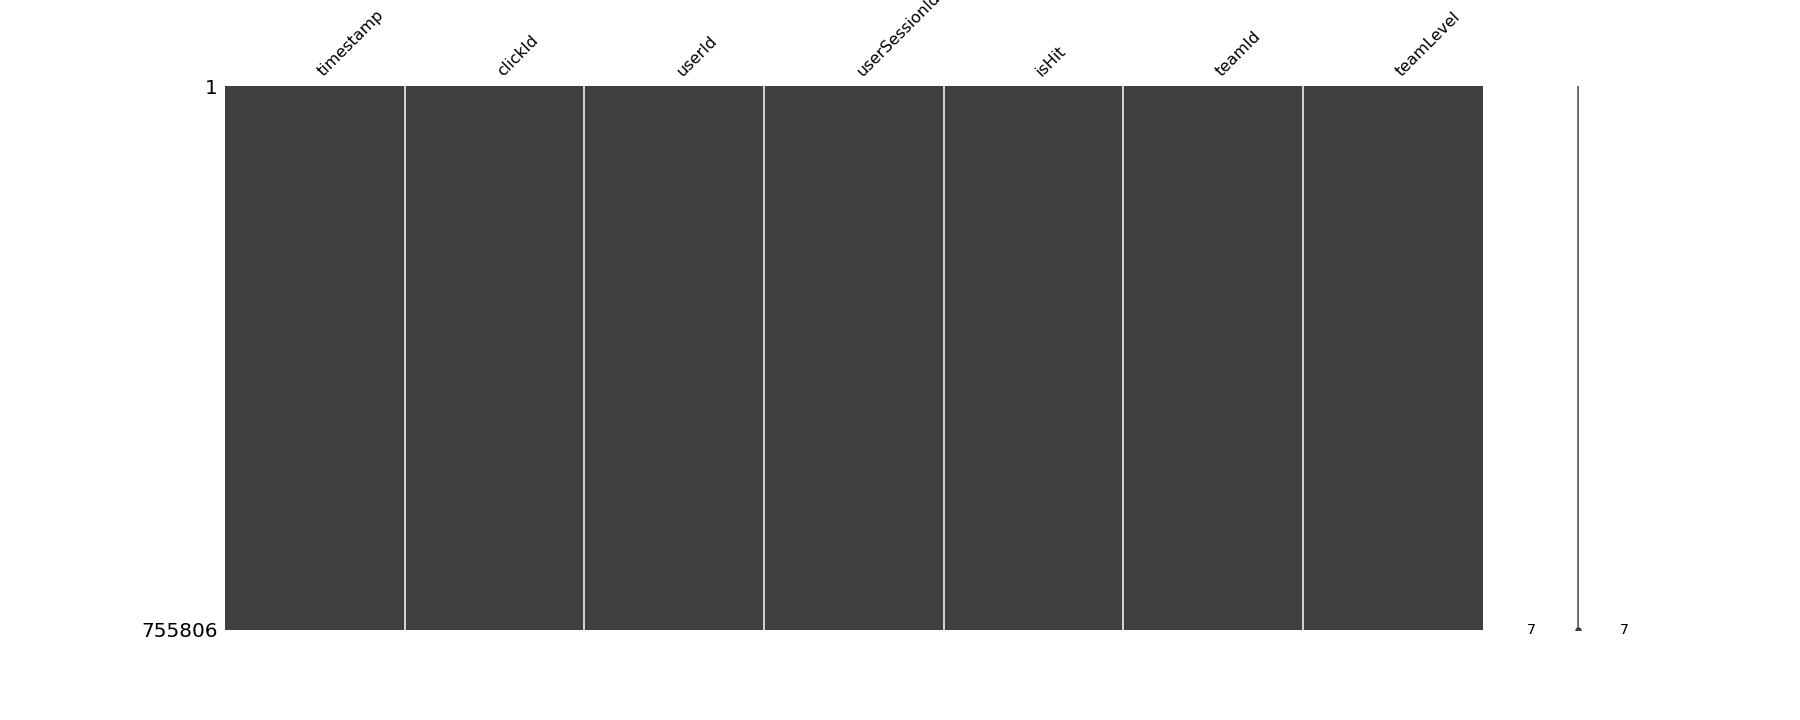
\includegraphics[scale=0.25]{img/Graphs/gameClicks/missingno_gameClicks.png}
\centering
\caption{missingno\_gameClicks}
\label{fig:missingno_gameClicks}
\end{figure}

Time series for game clicks again similar to previous graphs. The only difference is the line is much steeper.
\begin{figure}[H]
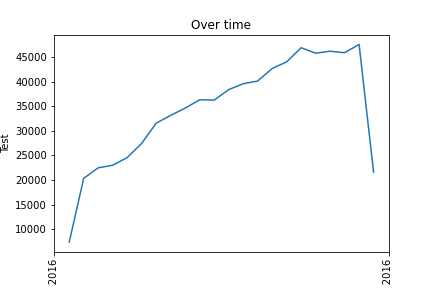
\includegraphics[scale=0.85]{img/Graphs/gameClicks/timeseries_gameClicks.png}
\centering
\caption{timeseries\_gameClicks}
\label{fig:timeseries_gameClicks}
\end{figure}